\chapter{Introducción}

Como bien es sabido, el desarrollo de una nueva aeronave partiendo de cero es un trabajo tremendamente complejo que supondría en la industria unos costes desmesurados. Por ello, en este Trabajo de Fin de Grado se plasmará el desarrollo de un diseño preliminar empleando, para ello, un análisis de vehículos semejantes ya existentes.

En este capítulo se tratarán, además de los objetivos del trabajo, las bases de la mecánica de vuelo de las aeronaves de ala rotatoria de forma sencilla.

\section{Objetivos del trabajo}

El objetivo principal de este trabajo será el diseño preliminar de un helicóptero no tripulado de peso máximo al despegue (MTOW, \emph{Maximum Take-off Weight}) de 450 kg al que se denominará \emph{DroneHE}.

Para ello, se desarrollará un modelo computacional basado en el de una aeronave tripulada ya existente. Dicho modelo requerirá seleccionar diversos parámetros de diseño que se decidirán en base a un análisis de las características de aeronaves similares que ya están desarrolladas. La escasez de datos hará necesario no limitar el análisis a helicópteros no tripulados y trabajar con un rango más amplio de modelos. Esta también es la causa por la que es necesario basar el modelo computacional del DroneHE en el de un helicóptero considerablemente más pesado.

Una vez se disponga del modelo, se procederá a resolver el problema del equilibrado de este, de manera que pueda obtenerse información acerca de sus actuaciones y comprobar la influencia de diversos parámetros de diseño en estas. Esto permitirá una optimización del diseño en etapas posteriores. El equilibrado se resolverá para:
\begin{itemize}
	\item Vuelo horizontal.
	\item Vuelo ascendente en espiral.
	\item Vuelo circular.
\end{itemize}
En cada uno de los casos se resolverá el problema para distintas cargas de pago.

\section{Uso de las aeronaves no tripuladas}
Las aeronaves no tripuladas (UAV, \textbf{U}nmanned \textbf{A}erial \textbf{V}ehicle) están fuertemente ligadas a la aviación militar, siendo esta industria la responsable principal de su desarrollo a lo largo de su historia.
Aunque anteriormente se dieron casos de UAV, como los globos con los que el ejército austriaco bombardeó Venecia en 1849, las primeras aeronaves no tripuladas como las conocemos hoy se desarrollaron durante la Primera Guerra Mundial por parte de los Estados Unidos.

A día de hoy, a pesar de que el desarrollo de la tecnología ha sido gracias a la industria militar, principalmente de la estadounidense, su uso se ha extendido más allá de esta. Ya no se trata de instrumentos de guerra ni de un artículo de lujo, sino que existe una gran variedad de aeronaves que cumplen distintas funciones fuera de la aviación militar, cuyo máximo exponente es la aviación comercial civil (algunos ejemplos son las aeronaves por radio control cuyo mando puede ser un \emph{smartphone} personal).

Algunos de estos usos son los siguientes:
\begin{itemize}
	\item Fotografía y grabación aérea, tanto profesional como recreativa.
	\item Valoración de daños en zonas afectadas por desastres.
	\item Transporte de mercancías.
	\item Seguimiento y predicción de fenómenos atmosféricos (tornados, tormentas, etc.)
	\item Control y patrullaje de fronteras.
	\item Inspecciones en zonas de difícil o imposible acceso.
	\item Entretenimiento.
\end{itemize}

Por otro lado, siguen creciendo los usos militares:
\begin{itemize}
	\item Combate aéreo.
	\item Supervisión y control.
	\item Vigilancia y reconocimiento de zonas.
	\item Señalización de objetivos.
\end{itemize}
Estos son solo algunos de los usos de los UAV, pero la lista crece continuamente.

Pese al fuerte desarrollo civil, el principal gasto mundial en aeronaves no tripuladas proviene del sector militar, debido al gasto que llevan consigo los programas militares y los costes de las aeronaves (en el año 2011 el coste del programa MQ-1 \emph{Predator} era de 2,38 mil millones de dólares \citep{Predatorunitbudget}, mientras que el coste de un solo aparato es de 4,03 millones de dólares \citep{Predatorprogrambudget}). Se espera que para el año 2020 el gasto global en aeronaves no tripuladas sea de 70 mil millones de dólares \citep{Goldman}.

Sin embargo, se prevé que haya un mayor crecimiento en el sector civil. Según datos de BI Intelligence, se estima un crecimiento del 19\% en el mercado civil frente a un 5\% en el militar para el período 2015-2020.
Esto se debe principalmente al incremento en la variedad de operaciones que los UAV son capaces de realizar y a su empleo por parte de las empresas. Debido a este crecimiento, se espera también la creación de 100 000 puestos de trabajo solo en los Estados Unidos para el 2025 \citep{AUVSI}.

\section{Mecánica del vuelo de un helicóptero}
%A completar posteriormente junto a lo anterior, de vez en cuando escribe algo mamon.
A modo de introducción, se hará un breve resumen de la mecánica del vuelo de un helicóptero. Si se desea profundizar en el tema o resolver cualquier duda que pudiese surgir durante la lectura, se recomienda acudir a \citet{Cuerva}, donde se desarrolla de forma más exhaustiva y completa.

\subsection{Sistemas de referencia}
En la física es muy importante definir correctamente los sistemas de referencia que se emplean en la resolución de cada problema, ya que las variables tendrán una forma u otra en función de en que sistema se definan.
En el caso de un helicóptero los sistemas de referencia principales son 4, a saber:
\begin{itemize}
	\item Ejes tierra $[O_{T};x_{T},y_{T},z_{T}]$
	\item Ejes cuerpo $[O;x,y,x]$
	\item Ejes árbol $[A;x_{A},y_{A},z_{A}]$
	\item Ejes pala $[E;x_{b},y_{b},z_{b}]$
\end{itemize}

El sistema de ejes tierra es aquel con origen $[O_{T}]$ en la superficie terrestre, $z_{T}$ apuntando en la dirección de la gravedad y $x_{T}$ e $y_{T}$ pertenecientes al plano tangente a la superficie terrestre y formando un triedro a derechas. En este sistema la posición del helicóptero queda definida por $\textbf{r}^{O}$ , siendo este el vector posición del centro de masas del helicóptero respecto al punto de referencia $O_{T}$.

El sistema de ejes cuerpo se define como el triedro a derechas con origen $O$ en el centro de masas de la aeronave y $x$ y $z$ en el plano central, con $x$ dirigido hacia hacia adelante y $z$ hacia abajo en una condición de vuelo normal. La importancia de este sistema radica en los ángulos de Euler, que son los ángulos que forman sus ejes con los ejes tierra, siendo estos:
\begin{itemize}
	\item Guiñada $\Psi$
	\item Cabeceo $\Theta$
	\item Balanceo $\Phi$
\end{itemize}

Estos ángulos se pueden definir como el giro del sistema de ejes cuerpo respecto al de ejes tierra, partiendo de una condición de paralelismo entre ambos, respecto a los ejes $z$, $y$ y $x$ respectivamente. Para facilitar su comprensión, se ha añadido el esquema \ref{AEuler} que representan dichos ángulos.
\begin{figure}[h]
	\centering
	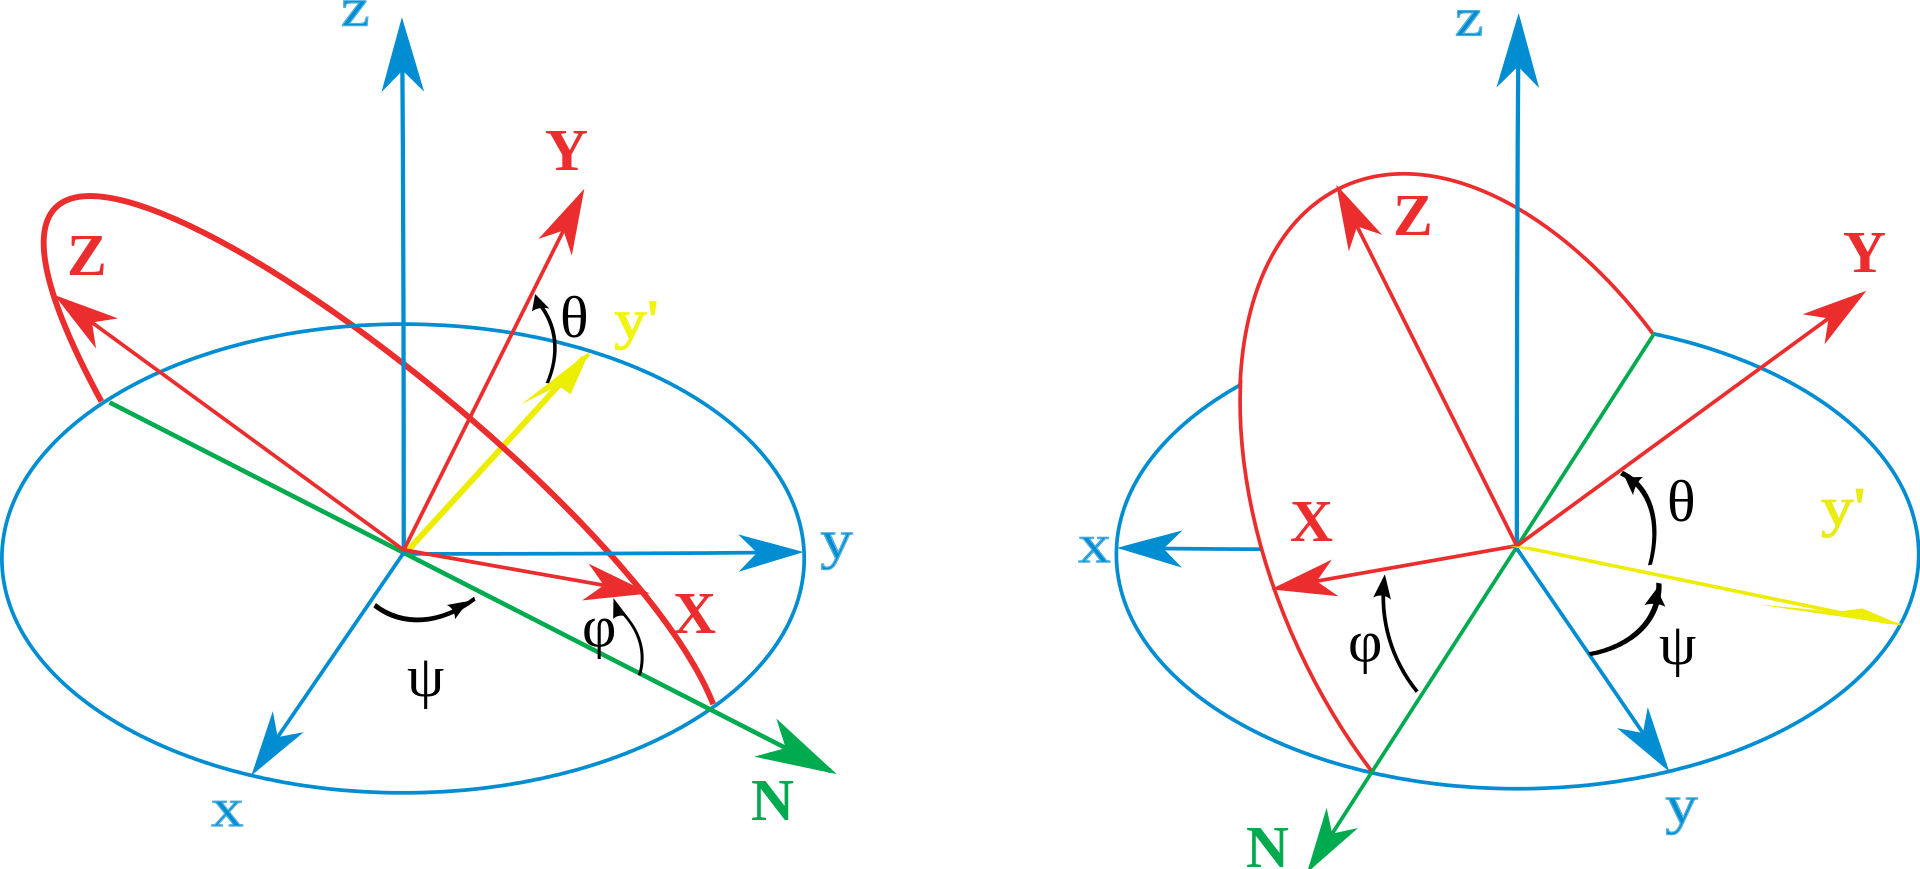
\includegraphics[width=110mm]{imagenes/AEuler}
	\caption{Representación de los ángulos de Euler, Guiñada, Cabeceo y Balanceo}
	\label{AEuler}
\end{figure}

El sistema de ejes árbol tiene su centro $A$ en la intersección del eje del rotor con el plano del rotor y sus ejes forman un triedro a derechas orientándose $z_{A}$ hacia el lado opuesto al fuselaje y $x$ hacia la parte trasera del helicóptero, perteneciendo al plano del rotor.

Por último, el sistema de ejes pala tiene su origen $E$ en la articulación de la pala. La dirección de $x_{b}$ es radial hacia la punta de la pala y la de $y_{b}$ es normal a ella, siendo $z_{b}$ tal que el triedro [$x_{b},y_{b},z_{b}$] sea a derechas.

Se puede apreciar que de estos 4 sistemas, los más relevantes para el estudio serán los de ejes tierra y cuerpo que sirven para describir la mecánica del vuelo de la aeronave, mientras que los ejes árbol y pala se reservan para el estudio aislado de la física del rotor y de las palas.\

Una vez definidos los sistemas de referencias se pueden empezar a plantear las ecuaciones.

\subsection{Ecuaciones del equilibrio}
Las primeras ecuaciones a considerar  son las de fuerzas y momentos, siendo estas:
\begin{equation}
\mathrm{\textbf{F}}^{ex}+M\mathrm{\textbf{g}}=\frac{\mathrm{d}(M\mathrm{\textbf{V}})}{\mathrm{d}t}=M\left(\frac{\mathrm{d\textbf{V}}}{\mathrm{d}t}\right)_{C}+M(\boldsymbol{\omega}\wedge\mathrm{\textbf{V}})
\label{EqF}
\end{equation}
\begin{equation}
\mathrm{\textbf{M}}^{ex}=\frac{\mathrm{d}([\mathrm{\textbf{I}}]\boldsymbol{\omega})}{\mathrm{d}t}=[\mathrm{\textbf{I}}]\left(\frac{\mathrm{d}\boldsymbol{\omega}}{\mathrm{d}t}\right)_C+\boldsymbol{\omega}\wedge[\mathrm{\textbf{I}}]\boldsymbol{\omega}
\label{EqM}
\end{equation}

Donde $\mathrm{\textbf{V}}(t)$ es una velocidad de vuelo cualquiera y $\boldsymbol{\omega}(t)$ la velocidad de giro de los ejes cuerpo respecto a los ejes tierra con $\mathrm{\textbf{F}}^{ex}$ y $\mathrm{\textbf{M}}^{ex}$ las fuerzas y momentos externos que actúan sobre el centro de gravedad del helicóptero (salvo el peso), $[\mathrm{\textbf{I}}]$ el tensor de inercia del vehículo, $M$ su masa y $\mathrm{\textbf{g}}$ el vector aceleración de la gravedad. El subíndice $C$ indica derivadas en ejes cuerpo, tal y como aparece en \citet{Cuerva}. Se han considerado $M$ e $[\mathrm{\textbf{I}}]$ constantes aunque en realidad no es así debido al consumo de combustible, pero se puede considerar que en el tiempo característico de una maniobra (segundos) el cambio es despreciable.\\

Tal y como se aprecia en (\ref{EqF}) y (\ref{EqM}), el vector de estado $\mathrm{\textbf{x}}(t)$ del sistema incluye las componentes de $\mathrm{\textbf{V}}(t)$ y $\boldsymbol{\omega}(t)$
en ejes cuerpo así como los ángulos de Euler $\Theta$, $\Psi$ y $\Phi$. Por otro lado, las magnitudes $\mathrm{\textbf{F}}^{ex}$ y $\mathrm{\textbf{M}}^{ex}$ pueden expresarse como funciones de las componentes del vector estado $\mathrm{\textbf{x}}(t)$ y sus derivadas $\mathrm{d\textbf{x}}(t)/\mathrm{d}t$, aunque también dependen de las magnitudes de control, agrupadas en el vector de control $\mathrm{\textbf{u}}(t)$ cuyas componentes son los ángulos de paso colectivo del rotor principal, paso cíclico longitudinal, paso cíclico lateral y paso colectivo del rotor antipar $\theta_0(t)$, $\theta_{1S}(t)$, $\theta_{1C}(t)$ y $\theta_T(t)$.
Cabe destacar que $\boldsymbol{\omega}(t)$ y los ángulos de Euler no son independientes, sino que están ligados por la relación cinemática:
\begin{equation}
	\boldsymbol{\omega}(t)=\omega_x\textbf{i}+\omega_y\textbf{j}+\omega_z\textbf{k}=\frac{\mathrm{d}\Psi}{\mathrm{d}t}\textbf{k}_T+\frac{\mathrm{d}\Theta}{\mathrm{d}t}\textbf{j}_{T1}+\frac{\mathrm{d}\Phi}{\mathrm{d}t}\textbf{i}_T
	\label{CinEuleromega}
\end{equation}

Y expresando el último término de la ecuación (\ref{CinEuleromega}) en ejes cuerpo, la ligadura cinemática se puede expresar con las siguientes ecuaciones:
\begin{equation}
	\boldsymbol{\omega}(t)=\left[
	\begin{array}{c}
	\omega_x\\
	\omega_y\\
	\omega_z
	\end{array}
	\right]=\left[	
	\begin{array}{ccc}
	0 & 1 & -\sin\Theta\\
	\cos\Phi & 0 & \sin\Phi\cos\Theta\\
	-\sin\Phi & 0 & \cos\Phi\cos\Theta
	\end{array}
	\right]\left[
	\begin{array}{c}
	\mathrm{d}\Theta/\mathrm{d}t\\
	\mathrm{d}\Phi/\mathrm{d}t\\
	\mathrm{d}\Psi/\mathrm{d}t
	\end{array}
	\right]
	\label{CinEuleromega2}
\end{equation}

Por tanto, las ecuaciones (\ref{EqF}), (\ref{EqM}) y (\ref{CinEuleromega2}) junto con las condiciones iniciales del vector estado $\mathrm{\textbf{x}_0}=\mathrm{\textbf{x}(0)}$ permiten conocer la evolución temporal del vector estado $\mathrm{\textbf{x}}(t)$ en función del vector de control $\mathrm{\textbf{u}}(t)$. En particular, conocidas las componentes del vector velocidad, se define el vector posición centro de masas tal que: 
\begin{equation}
	\mathrm{\textbf{r}^O}(t)=\int_{0}^{t}\mathrm{\textbf{V}}(t)\mathrm{d}t
\end{equation}
donde $\mathrm{\textbf{V}}(t)$ está expresada en ejes tierra ($u_T$, $v_T$, $w_T$). La trayectoria por tanto queda definida por el ángulo que forma el vector velocidad con la horizontal, $\gamma_T$ y el ángulo que forma con el plano vertical $y_T=0$, $\beta_T$, llamados respectivamente ángulo de inclinación de la trayectoria y ángulo de desviación lateral de la trayectoria, los cuales son:
\begin{equation}
	\gamma_T=\arctan\frac{-w_T}{\sqrt{u_T^2+v_T^2}}
	\label{gammat}
\end{equation}
y
\begin{equation}
\beta_T=\arctan\frac{v_T}{u_T}
\label{betat}
\end{equation}
siendo $\gamma_T$ positiva en vuelo ascendente, por ser entonces $w_T$ negativo por la definición de los ejes tierra.

\subsection{Acciones externas sobre el fuselaje}
Las acciones externas $\mathrm{\textbf{F}}^{ex}$ son un sumatorio de distintas componentes con distinto origen:
\begin{itemize}
	\item El rotor principal transmite al fuselaje la fuerza $\mathrm{\textbf{F}}^{rp}$ y el momento en $\mathrm{A}$, $\mathrm{\textbf{M}}^{rp}$.
	\item El rotor antipar transmite al fuselaje la fuerza $\mathrm{\textbf{F}}^{ra}$ y el momento en $\mathrm{A_a}$ (equivalente a A en el rotor principal), $\mathrm{\textbf{M}}^{ra}$.
	\item Las acciones aerodinámicas sobre el fuselaje se pueden modelizar como la fuerza $\mathrm{\textbf{F}}^{f}$ y el momento $\mathrm{\textbf{M}}^{f}$ sobre el punto de referencia $\mathrm{O_f}$.
	\item Las acciones aerodinámicas sobre los estabilizadores se pueden modelizar como las fuerzas $\mathrm{\textbf{F}}^{eh}$ y $\mathrm{\textbf{F}}^{ev}$, y los momentos $\mathrm{\textbf{M}}^{eh}$ y $\mathrm{\textbf{M}}^{ev}$ sobre los puntos de referencia $\mathrm{E_h}$ y $\mathrm{E_v}$ de las superficies de control.
\end{itemize}
pudiendo expresarse por tanto las fuerzas externas como:
\begin{equation}
	\mathrm{\textbf{F}}^{ex}=\mathrm{\textbf{F}}^{rp}+\mathrm{\textbf{F}}^{f}+\mathrm{\textbf{F}}^{ra}+\mathrm{\textbf{F}}^{eh}+\mathrm{\textbf{F}}^{ev}
\end{equation}
y los momentos externos como:
\begin{equation}
\begin{split}
	&\mathrm{\textbf{M}}^{ex}=\mathrm{\textbf{M}}^{rp}+\mathrm{\textbf{M}}^{f}+\mathrm{\textbf{M}}^{ra}+\mathrm{\textbf{M}}^{eh}+\mathrm{\textbf{M}}^{ev}+ \\
	&+\textbf{OA} \times \mathrm{\textbf{F}}^{rp}+\textbf{O}\textbf{O}_f \times \mathrm{\textbf{F}}^{f}+\textbf{OA}_a \times \mathrm{\textbf{F}}^{ra}+\\
	&+\textbf{OE}_h \times \mathrm{\textbf{F}}^{eh}+\textbf{OE}_v \times \mathrm{\textbf{F}}^{ev}
\end{split}
\end{equation}

Se puede observar que tanto las componentes de $\mathrm{\textbf{F}}^{ex}$ como de $\mathrm{\textbf{M}}^{ex}$ son de carácter aerodinámico, generadas por el rotor principal, el antipar, el fuselaje y las superficies estabilizadoras. Por tanto, será necesario modelizar estos elementos para poder realizar las simulaciones necesarias para el proyecto.

\subsection{Vuelo equilibrado}

Debido a la enorme complejidad de los cálculos anteriores y lo innecesario de su implementación para cumplir los objetivos de este proyecto, que son el cálculo de las actuaciones de un vehículo, se trabajará con un modelo simplificado: el del \emph{vuelo equilibrado}. Esto supone asumir que la resultante de las fuerzas externas que actúan sobre la aeronave es nula, lo que simplifica los cálculos sin afectar de forma relevante a los resultados de las actuaciones, prescindiendo de los cálculos para la estabilidad dinámica del sistema.
Esto también implica que:
\begin{itemize}
	\item La aceleración es nula, por lo que la velocidad de desplazamiento de la aeronave $\mathrm{\textbf{V}}(t)$ es constante.
	\item La aeronave no sufre cambios de actitud por lo que $\boldsymbol{\omega}(t)=0$.
\end{itemize}

Aplicando esto, las ecuaciones (\ref{EqF}) y (\ref{EqM}) se convierten en:
\begin{equation}
	\mathrm{\textbf{F}}^{ex}+M\mathrm{\textbf{g}}=0
	\label{EqFe}
\end{equation}
\begin{equation}
	\mathrm{\textbf{M}}^{ex}=0
	\label{EqMe}
\end{equation}
y la ligadura cinemática de la velocidad angular desaparece al volverse esta nula, por lo que el sistema se reduce a 10 incógnitas, el vector de estado de equilibrio $\mathrm{\textbf{x}}_e(u_e, v_e, w_e, \Theta_e, \Phi_e, \Psi_e)$ y las del vector de control de equilibrio $\mathrm{\textbf{u}}_e(\theta_{0e}, \theta_{1Se}, \theta_{1Ce}, \theta_{Te}$), y 6 ecuaciones.
Al resolver el problema aeromecánico (fuera del alcance de este documento) aparecen otras 3 ecuaciones:
\begin{equation}
\beta_0=\beta_0(\theta_0,\theta_{1S},\theta_{1C},\mu_{xA},\mu_{yA},\mu_{zA})
\label{beta0}
\end{equation}
\begin{equation}
\beta_{1C}=\beta_0(\theta_0,\theta_{1S},\theta_{1C},\mu_{xA},\mu_{yA},\mu_{zA})
\label{beta1c}
\end{equation}
\begin{equation}
\beta_{1S}=\beta_0(\theta_0,\theta_{1S},\theta_{1C},\mu_{xA},\mu_{yA},\mu_{zA})
\label{beta1s}
\end{equation}
donde se ha denominado $\mu_{xA}$,$\mu_{yA}$ y $\mu_{zA}$ a las componentes de la velocidad adimensionalizada con $\boldsymbol{\Omega}R$, lo que deja un total de 9 ecuaciones con 13 incógnitas.

Su resolución requeriría conocer de antemano 4 parámetros, pero si se le presta la debida atención al sistema (\ref{EqFe})-(\ref{beta1s}), en todo el mismo no aparece el ángulo de guiñada $\Psi_e$, por lo que la resolución no depende de él, y solo restaría conocer 3 variables del vector de estado o control para resolver el sistema, quedando este reducido a:
\begin{equation}
	F_x(\mathrm{\textbf{x}}_e^*,\mathrm{\textbf{u}}_e)-Mg\sin\Theta_e=0
\end{equation}
\begin{equation}
	F_y(\mathrm{\textbf{x}}_e^*,\mathrm{\textbf{u}}_e)+Mg\cos\Theta_e\sin\Phi_e=0
\end{equation}
\begin{equation}
	F_z(\mathrm{\textbf{x}}_e^*,\mathrm{\textbf{u}}_e)+Mg\cos\Theta_e\cos\Phi_e=0
\end{equation}
\begin{equation}
	M_z(\mathrm{\textbf{x}}_e^*,\mathrm{\textbf{u}}_e)=0
\end{equation}
\begin{equation}
	M_y(\mathrm{\textbf{x}}_e^*,\mathrm{\textbf{u}}_e)=0
\end{equation}
\begin{equation}
	M_x(\mathrm{\textbf{x}}_e^*,\mathrm{\textbf{u}}_e)=0
\end{equation}
donde $\mathrm{\textbf{x}}_e^*$ es el vector de estado sin incluir la velocidad angular ni el ángulo de guiñada \citep{Cuerva}.

\section{Cálculo de potencias}

Para el cálculo de la potencia necesaria para el vuelo se puede optar por dos métodos: el \emph{método de la energía} y el \emph{método del equilibrado}. El \emph{método de la energía} resulta más simple en los cálculos, pues el \emph{método del equilibrado} requiere de la solución del propio equilibrado del helicóptero primero. Estos cálculos resultan bastante más complejos, pero como para realizar los cálculos del vuelo se resolverán igualmente, resulta más conveniente usar este último método.

Una vez resuelto el equilibrado del vehículo, el cálculo de potencias resulta sencillo al haber calculado las fuerzas sobre los elementos de la aeronave, pues ese mismo cálculo permite conocer el par que se ha de aplicar al árbol de los rotores. Para el caso del rotor principal este par se denomina $Q_{rp}$, y a través del régimen de giro del rotor se puede obtener la potencia necesaria $P_{rp}=\Omega Q_{rp}$. De forma análoga, se procede al cálculo en el rotor antipar para obtener $P_{ra}$.

Por último, es necesario modelizar de alguna forma las pérdidas en las trasmisiones que se hará mediante la definición de los factores $\eta_{Trp}$ y $\eta_{Tra}$, que se definen como la relación entre la potencia disipada en la trasmisión del rotor (principal o antipar) y la potencia suministrada al mismo.

Aunque no se expondrá en este trabajo, una explicación del método de la energía puede encontrarse en \citet{Cuerva}.

\section[\textbf{HE}licopter and \textbf{RO}tor \textbf{E}quilibrium and \textbf{S}tability toolbox]{HEROES}

%Por aquí explicar que no se harán cálculos directamente, sino que se usará la herramienta. Descripción, sistema de "cajas", incógnitas de los problemas, soluciones...
Para el cálculo de las actuaciones de la aeronave se empleará HEROES (\textbf{HE}licopter and \textbf{RO}tor \textbf{E}quilibrium and \textbf{S}tability toolbox).
HEROES es una herramienta de MATLAB desarrollada en conjunto por profesores y alumnos de la Escuela Técnica Superior de Ingeniería Aeronáutica y del Espacio de la Universidad Politécnica de Madrid, principalmente del departamento de Aeronaves y Vehículos Espaciales.

Esta herramienta permite un cálculo rápido del equilibrado de un helicóptero (entre otras muchas funciones). Es muy importante saber distinguir en esta herramienta cuáles son las variables de entrada del problema y las de salida. Esto, que en primera instancia puede parecer sencillo, requiere un nivel de comprensión alto de la mecánica del vuelo de un helicóptero.

Para el caso del equilibrado las variables de entrada principales serán el modelo de atmósfera, la altitud, el modelo del vehículo y las condiciones de vuelo del mismo. HEROES, con los datos aportados, generará un modelo adimensional y resolverá las ecuaciones del equilibrado para después dimensionalizar los resultados. Estos resultados son las variables de salida y entre muchas otras se encuentran las potencias de los rotores, las fuerzas y momentos aerodinámicos y los controles del helicóptero.

Además, esta herramienta permite generar modelos para helicópteros a partir de un modelo ya existente y los siguientes datos de diseño del nuevo helicóptero:

\begin{itemize}
	\item Número de palas del rotor principal.
	\item Radio del rotor principal.
	\item Velocidad de giro del rotor principal.
	\item Peso de la aeronave.
	\item Número de palas del rotor antipar.
\end{itemize}

Junto a estos datos son necesarios datos atmosféricos, como la densidad atmosférica que la herramienta obtiene a través de un modelo atmosférico y una altitud dada.

El proceso que sigue la herramienta es una adimensionalización del modelo existente para posteriormente dimensionalizarlo de nuevo usando para ello las características de la nueva aeronave. Todo este proceso se explicará con más detalle posteriormente.

\section{Misión del DroneHE}

Para finalizar con la introducción, es necesario definir una misión para la aeronave que permita optimizar el diseño a la misma.
Este DroneHE será un vehículo de vigilancia y búsqueda, por lo que será necesario embarcar un sistema de cámaras según los requisitos concretos del usuario, además de contar con una autonomía que permita mantener el helicóptero en servicio todo el tiempo posible.

